% !TEX program = xelatex
\documentclass[a4paper, 10]{article}
% include some packages
\usepackage{graphicx, color, pgfplots, pgf-umlsd, ifthen}
\usepackage{float}
\usepackage[]{fp}
\usepackage{amsmath, amsfonts, amssymb}
\usepackage{tikz}
\usepackage[UTF8]{ctex}
\usepackage{hyperref}
\usepackage{xcolor}

% Change settings for caption
\renewcommand{\figurename}{Figure}
\renewcommand{\tablename}{Table}

% Path for my images
\graphicspath{{./images/}}

% Settings for the neural network plots
\usetikzlibrary{matrix, patterns, spy, fit, calc}
\usepgfplotslibrary{groupplots}
\pgfplotsset{compat=newest}
\FPset{totalOffset}{0}

% A new command to draw the neural network
\newcommand{\networkLayer}[9] {
	% Define the macro.
	% 1st argument: Height and width of the layer rectangle slice.
	% 2nd argument: Depth of the layer slice
	% 3rd argument: X Offset --> use it to offset layers from previously drawn layers.
	% 4th argument: Y Offset --> Use it when an output needs to be fed to multiple layers that are on the same X offset.
	% 5th argument: Z Offset --> Use to offset layers from previous 
	% 6th argument: Options for filldraw.
	% 7th argument: Text to be placed below this layer.
	% 8th argument: Name of coordinates. When name = "start" this resets the offset counter
	% 9th argument: list of nodes to connect to (previous layers)
	% 全局变量
	\xdef\totalOffset{\totalOffset}
 	\ifthenelse{\equal{#8} {start}}
 	{\FPset{totalOffset}{0}}
 	{}
 	\FPeval\currentOffset{0+(totalOffset)+(#3)}

	\def\hw{#1} % Used to distinguish input resolution for current layer.
	\def\b{0.02}
	\def\c{#2} % Width of the cube to distinguish number of input channels for current layer.
	\def\x{\currentOffset} % X offset for current layer.
	\def\y{#4} % Y offset for current layer.
	\def\z{#5} % Z offset for current layer.
	\def\inText{#7}
    % Define references to points on the cube surfaces
    \coordinate (#8_front) at  (\x+\c  , \z      , \y);
    \coordinate (#8_back) at   (\x     , \z      , \y);
    \coordinate (#8_top) at    (\x+\c/2, \z+\hw/2, \y);
    \coordinate (#8_bottom) at (\x+\c/2, \z-\hw/2, \y);
    
 	% Define cube coords
	\coordinate (blr) at (\c+\x,  -\hw/2+\z,  -\hw/2+\y); %back lower right
	\coordinate (bur) at (\c+\x,   \hw/2+\z,  -\hw/2+\y); %back upper right
	\coordinate (bul) at (0 +\x,   \hw/2+\z,  -\hw/2+\y); %back upper left
	\coordinate (fll) at (0 +\x,  -\hw/2+\z,   \hw/2+\y); %front lower left
	\coordinate (flr) at (\c+\x,  -\hw/2+\z,   \hw/2+\y); %front lower right
	\coordinate (fur) at (\c+\x,   \hw/2+\z,   \hw/2+\y); %front upper right
	\coordinate (ful) at (0 +\x,   \hw/2+\z,   \hw/2+\y); %front upper left
	

    % Draw connections from other points to the back of this node
    \ifthenelse{\equal{#9} {}}
 	{} % 为空什么都不做
 	{ % 非空 开始画层与层之间的连线
 	    \foreach \val in #9
 	    % \val = start_front
 	        \draw[line width=0.3mm] (\val)--(#8_back);
 	}
 	
	% Draw the layer body.
	% back plane
	\draw[line width=0.3mm](blr) -- (bur) -- (bul);
	% front plane
	\draw[line width=0.3mm](fll) -- (flr) node[midway,below] {\inText} -- (fur) -- (ful) -- (fll);
	\draw[line width=0.3mm](blr) -- (flr);
	\draw[line width=0.3mm](bur) -- (fur);
	\draw[line width=0.3mm](bul) -- (ful);

	% Recolor visible surfaces
	% front plane
	\filldraw[#6] ($(fll)+(\b,\b,0)$) -- ($(flr)+(-\b,\b,0)$) -- ($(fur)+(-\b,-\b,0)$) -- ($(ful)+(\b,-\b,0)$) -- ($(fll)+(\b,\b,0)$);
	\filldraw[#6] ($(ful)+(\b,0,-\b)$) -- ($(fur)+(-\b,0,-\b)$) -- ($(bur)+(-\b,0,\b)$) -- ($(bul)+(\b,0,\b)$);

	% Colored slice.
	\ifthenelse {\equal{#6} {}}
	{} % Do not draw colored slice if #6 is blank.
	% Else, draw a colored slice.
	{\filldraw[#6] ($(flr)+(0,\b,-\b)$) -- ($(blr)+(0,\b,\b)$) -- ($(bur)+(0,-\b,\b)$) -- ($(fur)+(0,-\b,-\b)$);}

	\FPeval\totalOffset{0+(currentOffset)+\c}
}
% infos about the doc
\begin{document}
\title{HW2: Convolutional Autoencoder}
\author{王昊文}

\maketitle


% Document starts here
\section{Overview}
    In this homework, I will be training a simple autoencoder, that will 
    extract latent codes of the \textbf{Wafer map} dataset. Our goal is to 
    generate simialr images to the wafer dataset, by adding Gaussian noise
    into the latent code. \\
    \indent The whole homework strictly follows the object-orientated philosophy, which 
    treats \emph{datatset}, \emph{data loader}, \emph{trainer}, \emph{logger} as 
    different objects, so that it can be very convinient to write your own custom
    objects. You can combine all your settings and put them under \verb|config.json|
    inside the root folder. \\ 
    \indent Also, you will find that the structure is highly similar to 
    \href{https://github.com/victoresque/pytorch-template}{pytorch template},
    which allows me to have a basic building block to build this project.
    
\section{Details}
    \subsection{Data}
        In the Wafer dataset, we have a total of 1281 of data, testing
        data is not required in this project since we have to generate
        images directly from the training data. \\
        \indent Each image has a height and width of 26, and each image 
        contains three channels, however the three channels does not
        indicate RGB, but denotes whether the region is \emph{defected}
        , \emph{normal} or it is the \emph{boundary} of the wafer. Each
        channel can only be boolean values, that is, only 0 or 1, to 
        indicate the status of the area under. \\
        \indent There are 10 types of the wafer, there will be an obvious
        architecture between the 10 types of wafer. We will demonstrate
        the results from 10 different types of wafer in the result
        section.

    \subsection{Model}
        \subsubsection{Intuition and loss function selection} 
            Recall that our task is to generate similar images by adding
            Gaussian noise into the latent code generated by the autoencoder.
            Hence, when training, we try to let the output image be identical
            to the input image. Note that the model can be easily learning
            identity if our encoder and decoder have the same architecture, hence
            we must use an appropriate architecture design for our encoder and decoder. \\
            \indent In this case, for image data, convolution neural network on the decoder
            side and transpose-convolution at the encoder side fits well for this task.
            Since we are trying to match the input and output image, \textbf{MSE loss}
            will be used in this homework.
        \subsubsection{Architecture} 
            The model architecture is shown in figure \ref{fig:cnn}. Note that is defined
            under \verb|model.py|.\\
            \indent In figure \ref{fig:cnn}, the yellow module shows a convolution or a 
            transpose-convolution(for convinience, I denoted it as DeConv). Each convolution
            and transpose-convolution has a stride of 1 and a kernel size of 3, by setting it
            this way, we can prevent the shape from decreasing. One thing to note is that
            we will add a maxpooling at the decoder side and an upsampling at the encoder
            to form a structure for autoencoders, hence at every convolution/transpose-convolution,
            I will increase/decrease the output channel, to preserve more information
            with response to the decrease/increase of the output size. \\
            \indent The blue module denotes either a Maxpooling or upsampling module.
            More details are listed in table \ref{table:1}.
            \begin{table}[h!]
                \centering
                \begin{tabular}{|c|c|c|}
                    \hline
                    Layer               &   Output Shape               & Param Num. \\
                    \hline
                    Conv2d-1            &   [128, 16, 26, 26]          & 448 \\
                    BatchNorm2d-2       &   [128, 16, 26, 26]          & 32 \\
                    ReLU-3              &   [128, 16, 26, 26]          & 0 \\
                    Conv2d-4            &   [128, 32, 26, 26]          & 4,640 \\
                    BatchNorm2d-5       &   [128, 32, 26, 26]          &    64 \\
                    ReLU-6              &   [128, 32, 26, 26]          &     0 \\
                    Conv2d-7            &   [128, 64, 26, 26]          &18,496 \\
                    BatchNorm2d-8       &   [128, 64, 26, 26]          &   128 \\
                    ReLU-9              &   [128, 64, 26, 26]          &     0 \\
                    MaxPool2d-10        &   [128, 64, 13, 13]          &     0 \\
                    ConvTranspose2d-11  &   [128, 32, 13, 13]          &18,464 \\
                    BatchNorm2d-12      &   [128, 32, 13, 13]          &    64 \\
                    ReLU-13             &   [128, 32, 13, 13]          &     0 \\
                    ConvTranspose2d-14  &   [128, 16, 13, 13]          & 4,624 \\
                    BatchNorm2d-15      &   [128, 16, 13, 13]          &    32 \\
                    ReLU-16             &   [128, 16, 13, 13]          & 0     \\
                    Interpolate-17      &   [128, 16, 26, 26]          & 0     \\
                    ConvTranspose2d-18  &   [128, 3, 26, 26]           & 435   \\
                    BatchNorm2d-19      &   [128, 3, 26, 26]           & 6     \\
                    ReLU-20             &   [128, 3, 26, 26]           & 0    \\
                    \hline
                \end{tabular}
                \caption{A list of the layers of the current model}
                \label{table:1}
            \end{table}

        \begin{figure}
            \centering
            \noindent\resizebox{\textwidth}{!}{
            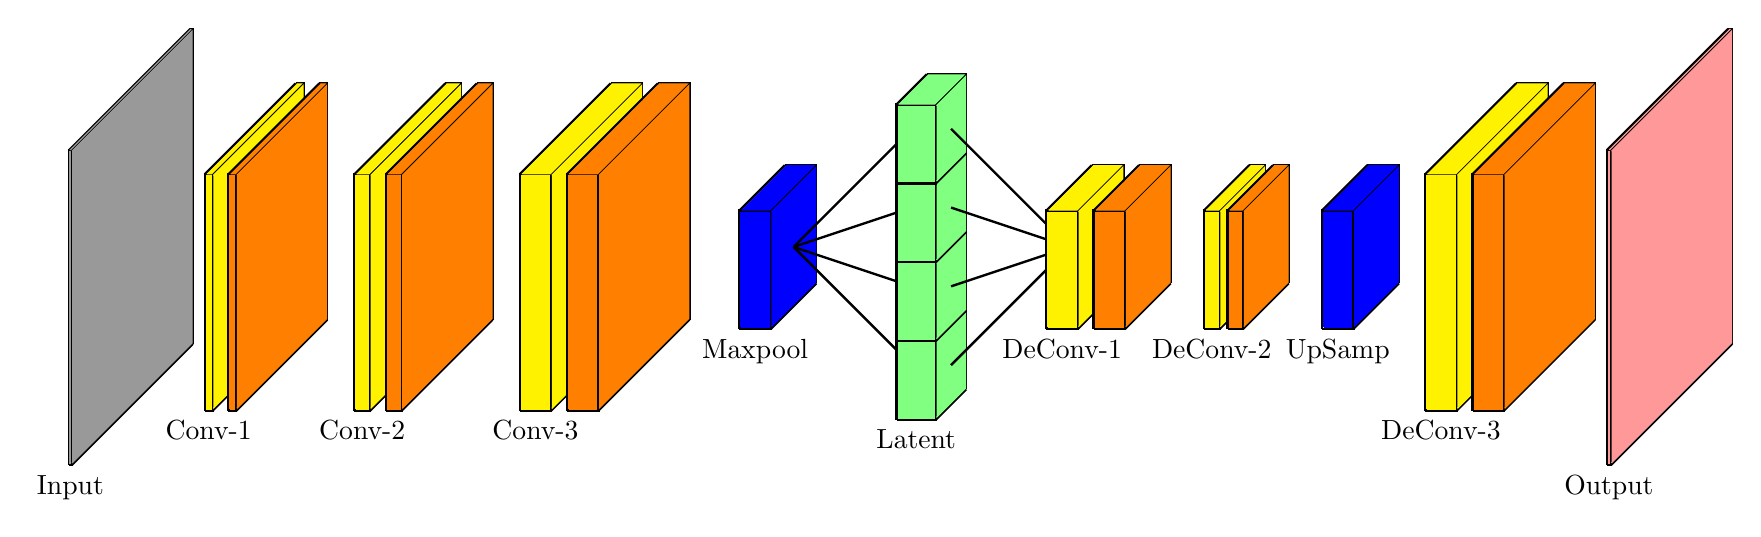
\begin{tikzpicture}
                % INPUT
                \networkLayer{4.0}{0.03}{0.0}{0.0}{0.0}{color=gray!80}{Input}{input}{}
                % ENCODER
                \networkLayer{3.0}{0.1}{1.5}{0.0}{0.0}{color=yellow}{Conv-1}{}{}    % S1
                \networkLayer{3.0}{0.1}{0.2}{0.0}{0.0}{color=orange}{}{}{}        % S2
                \networkLayer{3.0}{0.2}{1.5}{0.0}{0.0}{color=yellow}{Conv-2}{}{}    % S1
                \networkLayer{3.0}{0.2}{0.2}{0.0}{0.0}{color=orange}{}{}{}        % S2
                \networkLayer{3.0}{0.4}{1.5}{0.0}{0.0}{color=yellow}{Conv-3}{}{}    % S1
                \networkLayer{3.0}{0.4}{0.2}{0.0}{0.0}{color=orange}{}{}{}        % S2
                % \networkLayer{1.5}{0.8}{0.1}{0.0}{0.0}{color=white}{conv}{}{}    % S1
                % \networkLayer{1.5}{0.8}{0.1}{0.0}{0.0}{color=white}{}{}{}        % S2
                % \networkLayer{1.0}{1.5}{0.1}{0.0}{0.0}{color=white}{conv}{}{}    % S1
                \networkLayer{1.5}{0.4}{1.5}{0.0}{0.0}{color=blue}{Maxpool}{mid}{}        % S2

                \networkLayer{1.0}{0.5}{1.5}{0.0}{-1.5}{color=green!50}{Latent}{bot}{{mid_front}}
                \networkLayer{1.0}{0.5}{-0.5}{0.0}{-0.5}{color=green!50}{}{bot_1}{{mid_front}}
                \networkLayer{1.0}{0.5}{-0.5}{0.0}{0.5}{color=green!50}{}{top_1}{{mid_front}}
                \networkLayer{1.0}{0.5}{-0.5}{0.0}{1.5}{color=green!50}{}{top}{{mid_front}}
                % \networkLayer{1.0}{0.5}{1.5}{0.0}{0.0}{color=blue!50}{sum}{}{{bot_front,top_front}}

                % DECODER
                \networkLayer{1.5}{0.4}{1.5}{0.0}{0.0}{color=yellow}{DeConv-1}{}{{bot_front, bot_1_front, top_front, top_1_front}} % S1
                \networkLayer{1.5}{0.4}{0.2}{0.0}{0.0}{color=orange}{}{}{}       % S2
                \networkLayer{1.5}{0.2}{1.0}{0.0}{0.0}{color=yellow}{DeConv-2}{}{} % S1
                \networkLayer{1.5}{0.2}{0.1}{0.0}{0.0}{color=orange}{}{}{}       % S2
                \networkLayer{1.5}{0.4}{1.0}{0.0}{0.0}{color=blue}{UpSamp}{}{}        % S2
                \networkLayer{3.0}{0.4}{1.2}{0.0}{0.0}{color=yellow}{DeConv-3}{}{}       % S1
                \networkLayer{3.0}{0.4}{0.2}{0.0}{0.0}{color=orange}{}{}{{}}       % S2

                % OUTPUT
                \networkLayer{4.0}{0.05}{1.5}{0.0}{0.0}{color=red!40}{Output}{}{}     % Pixelwise segmentation with classes.
            \end{tikzpicture}
            }
            \caption{High-level of our model architecture}
            \label{fig:cnn}
        \end{figure}
    \subsection{Training and validation}
            As shown in figure \ref{fig:2}, the loss curve is plot via 
            tensorboard. Note that the horizontal axis is drawn in 
            unit of steps. When training, I set the batch size 
            to 128. Since there are 1281 samples of the training data,
            that is approximately 11 steps for epoch, and this curve
            is drawn in total of 150 epochs, that is around 1.6k steps.
            During training, I used adam as the optimizer, with weight decay
            of 0.001. Also, the learning rate is scheduled to decay at a 
            rate of 0.5 for every 40 epoch, in order to further decrease
            the loss value.
    \begin{figure}[J]
        \centering
        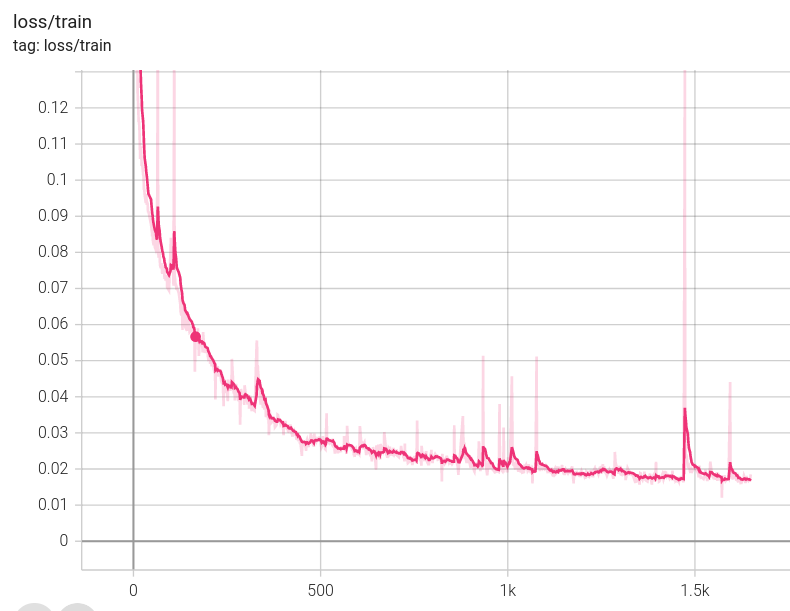
\includegraphics[scale=0.5]{Learning-Curve1.png}
        \caption{The MSE loss curve of the model} \label{fig:2}
    \end{figure}
    \subsection{Performace}
        I have provided a best model \verb|checkpoint-epoch300.pth| and the config 
        \verb|config.json| under the root folder. You can easily visualize 
        the results by using the \verb|test.py| given under the root folder.
        Several images are already stored in \verb|img/| folder, you can 
        see the quality of the image generated is pretty good.
\section{Result Visualization}
    \begin{figure}[H]
        \centering
        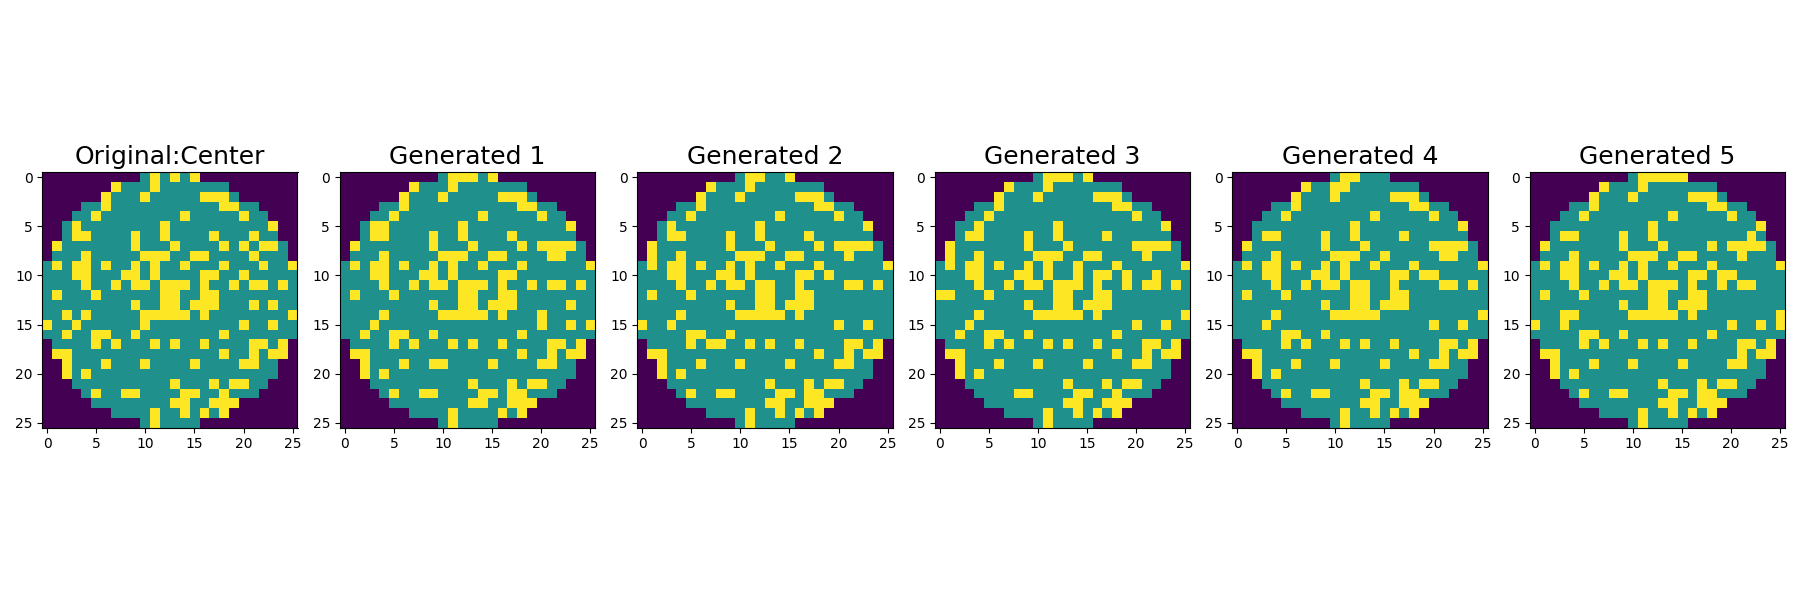
\includegraphics[width=\textwidth]{Center.png}
        \caption{Center} \label{fig:4}
    \end{figure}
    \begin{figure}[H]
        \centering
        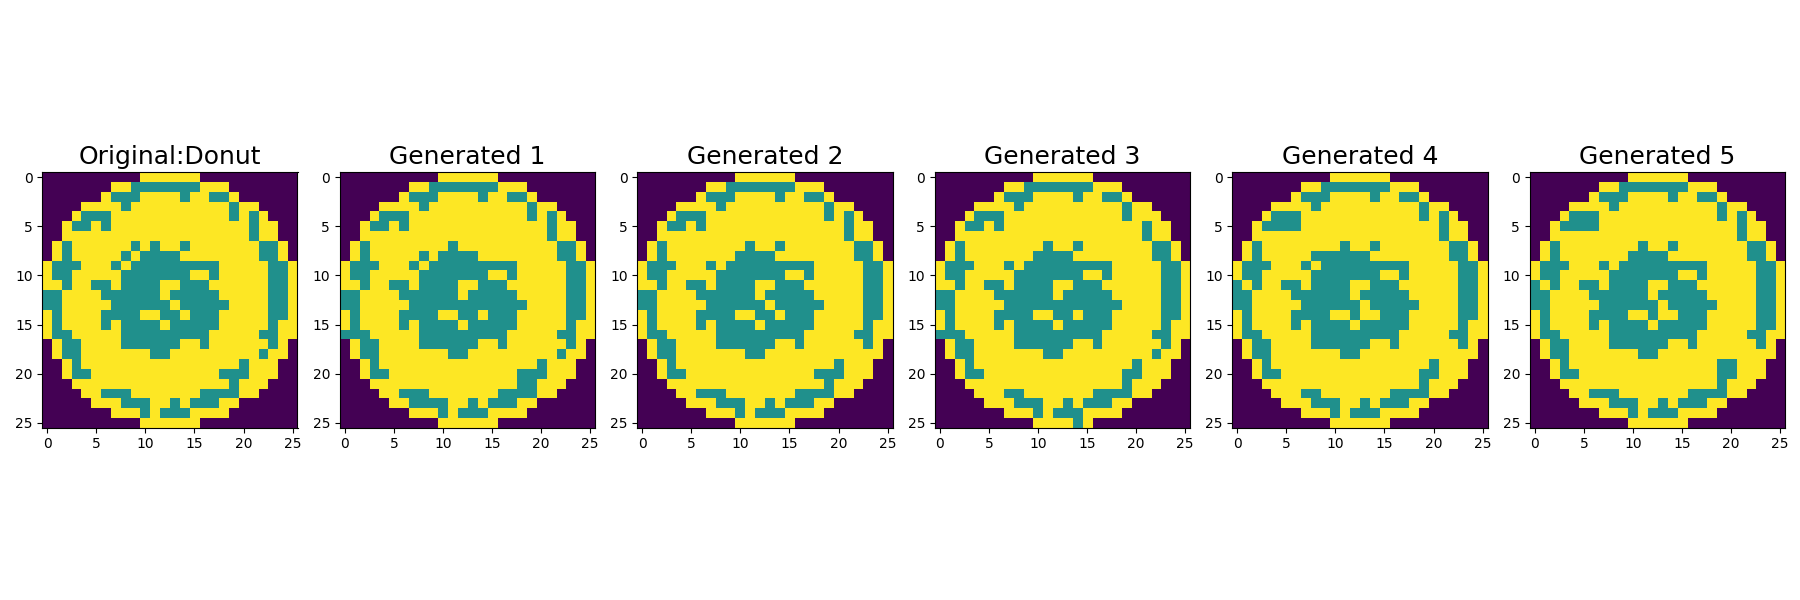
\includegraphics[width=\textwidth]{Donut.png}
        \caption{Donut} \label{fig:5}
    \end{figure}
    \begin{figure}[H]
        \centering
        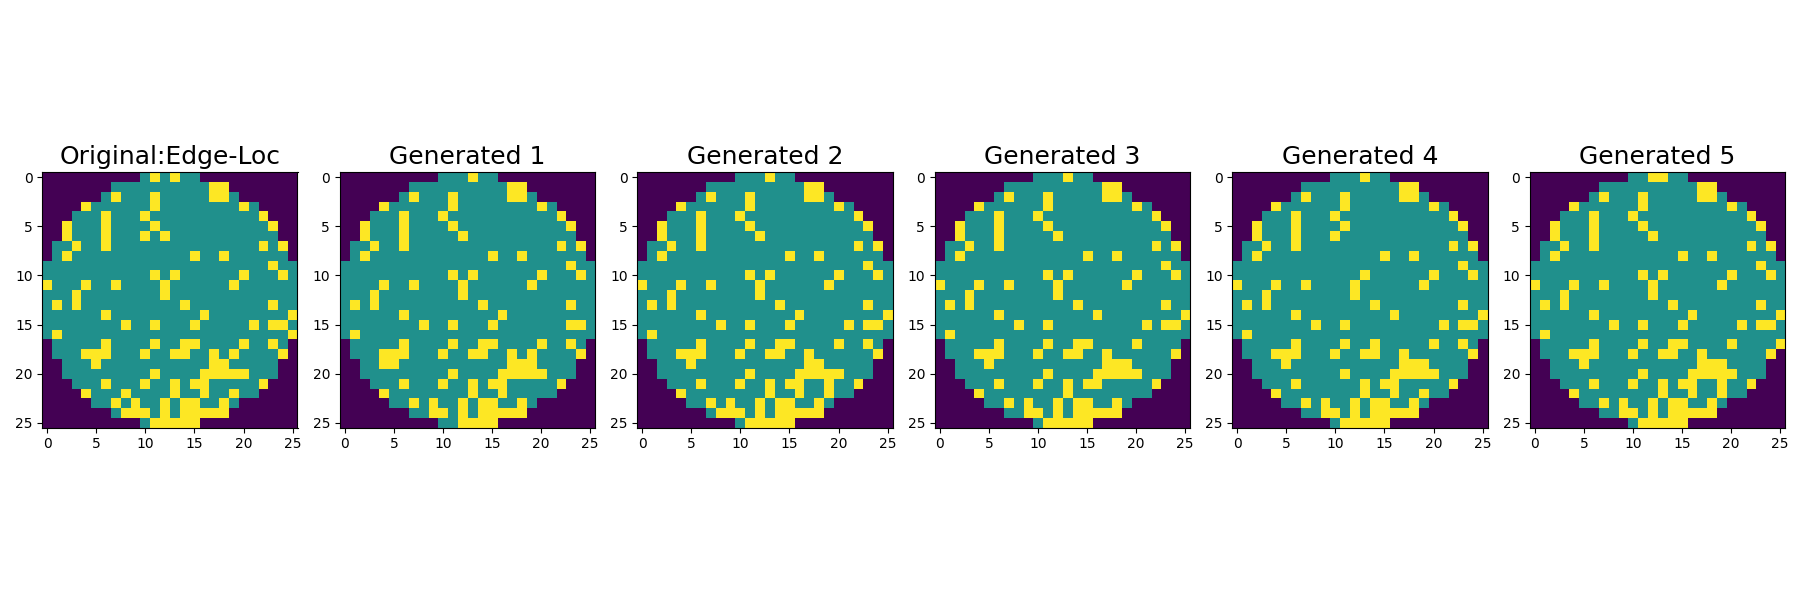
\includegraphics[width=\textwidth]{Edge-Loc.png}
        \caption{Edge-Loc} \label{fig:6}
    \end{figure}
    \begin{figure}[H]
        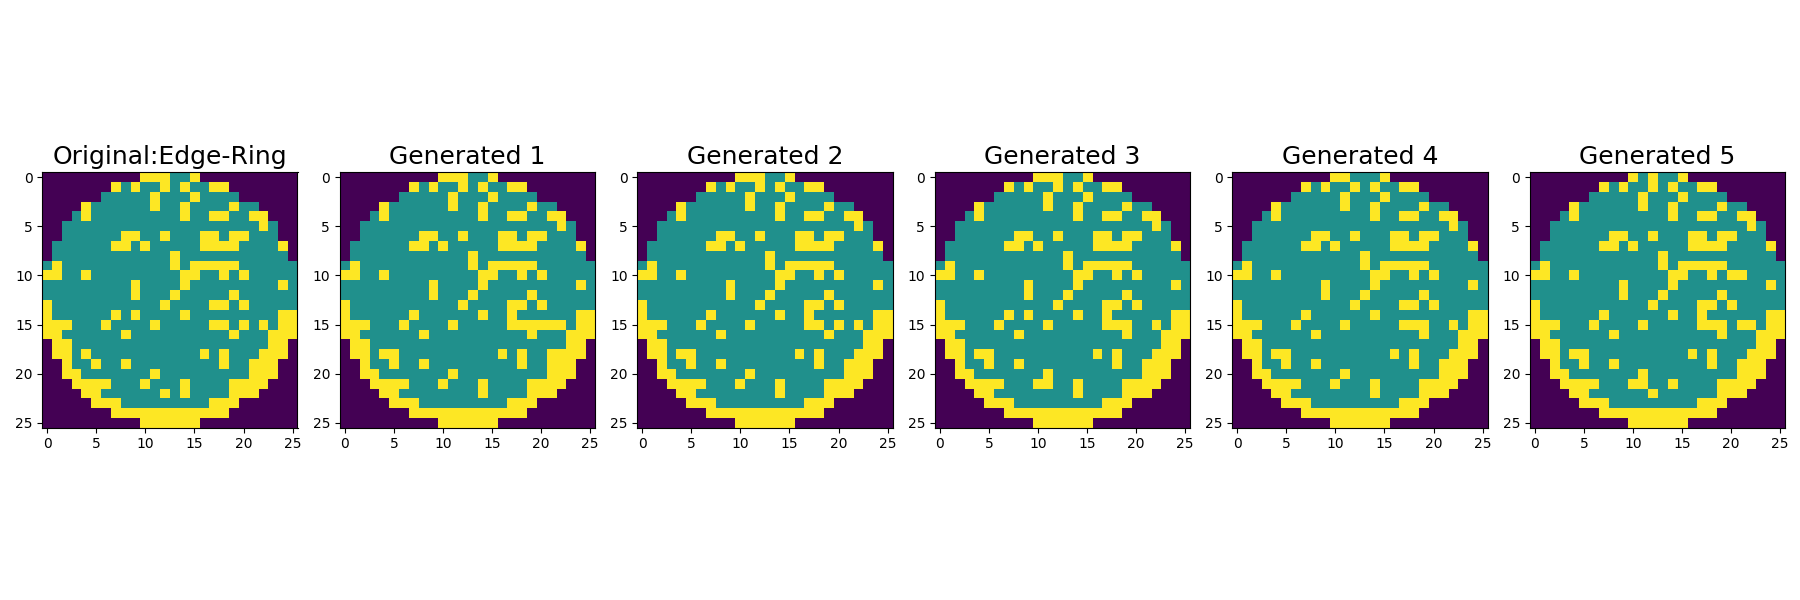
\includegraphics[width=\textwidth]{Edge-Ring.png}
        \centering
        \caption{Edge-Ring} \label{fig:7}
    \end{figure}
    \begin{figure}[H]
        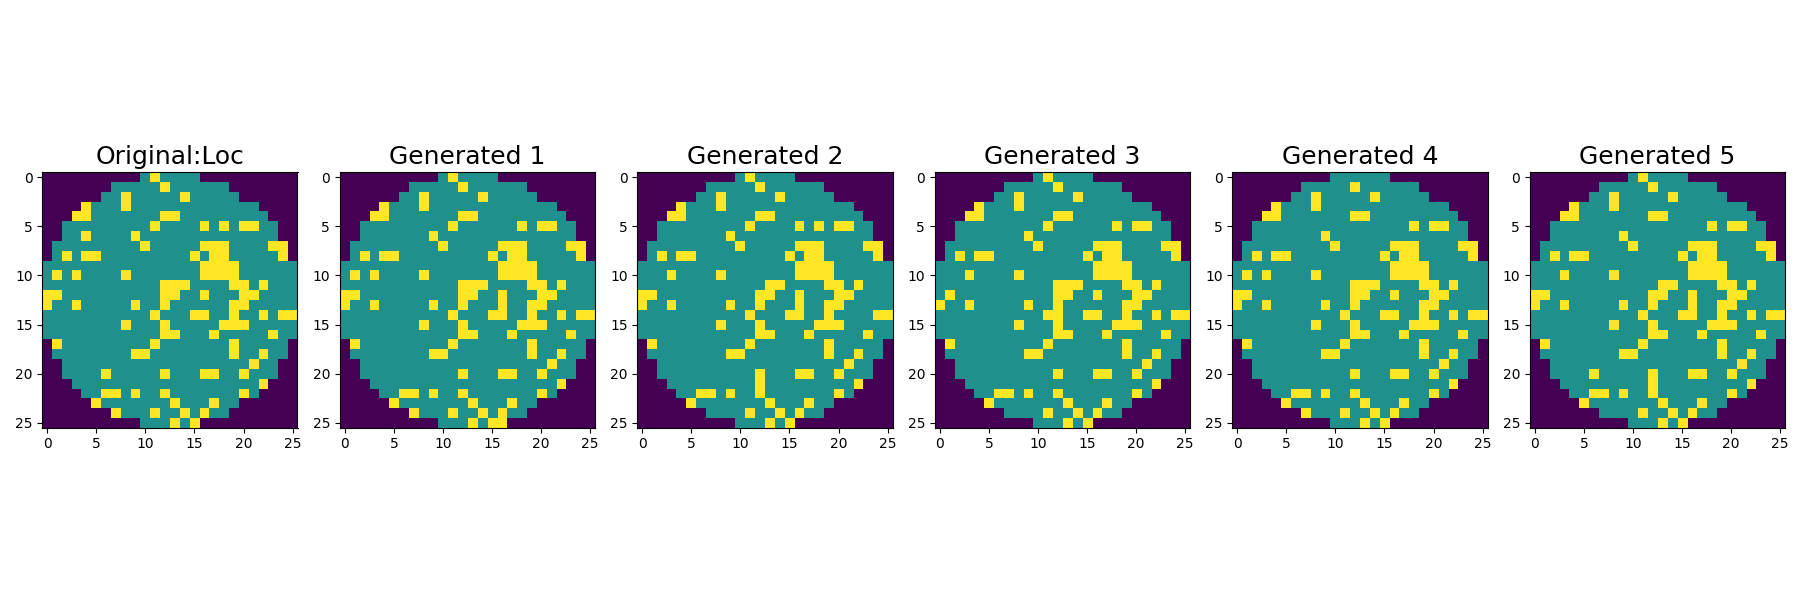
\includegraphics[width=\textwidth]{Loc.png}
        \centering
        \caption{Loc} \label{fig:8}
    \end{figure}
    \begin{figure}[H]
        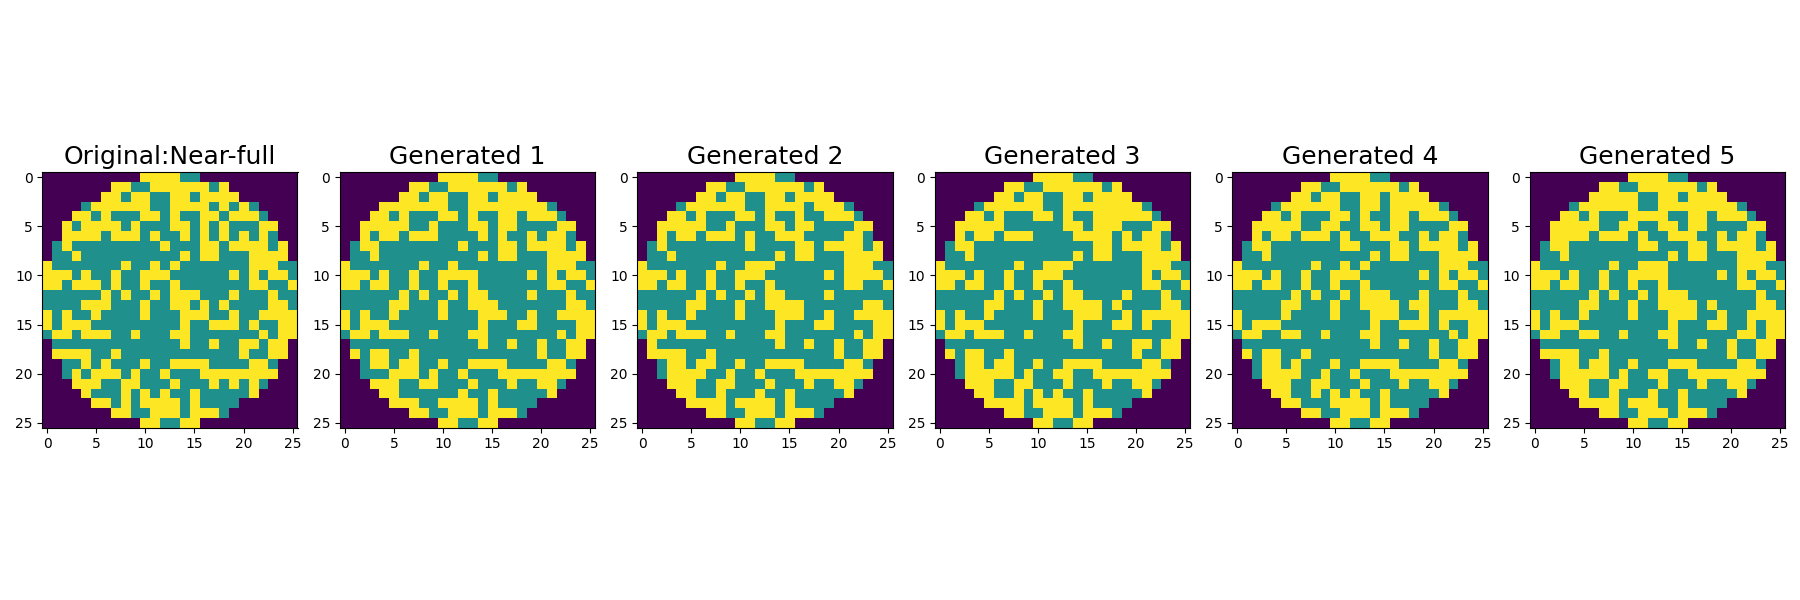
\includegraphics[width=\textwidth]{Near-full.png}
        \centering
        \caption{Near-full} \label{fig:9}
    \end{figure}
    \begin{figure}[H]
        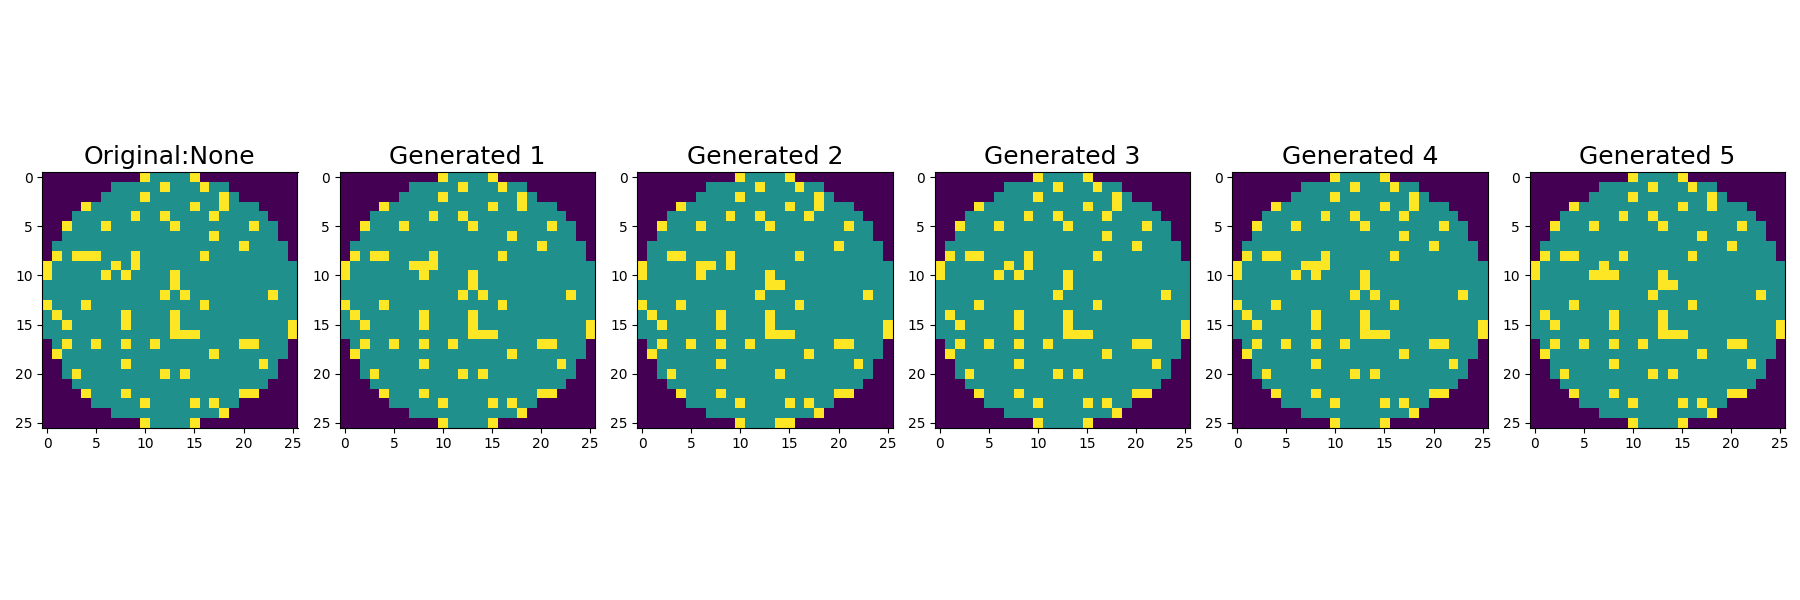
\includegraphics[width=\textwidth]{None.png}
        \centering
        \caption{None} \label{fig:10}
    \end{figure}
    \begin{figure}[H]
        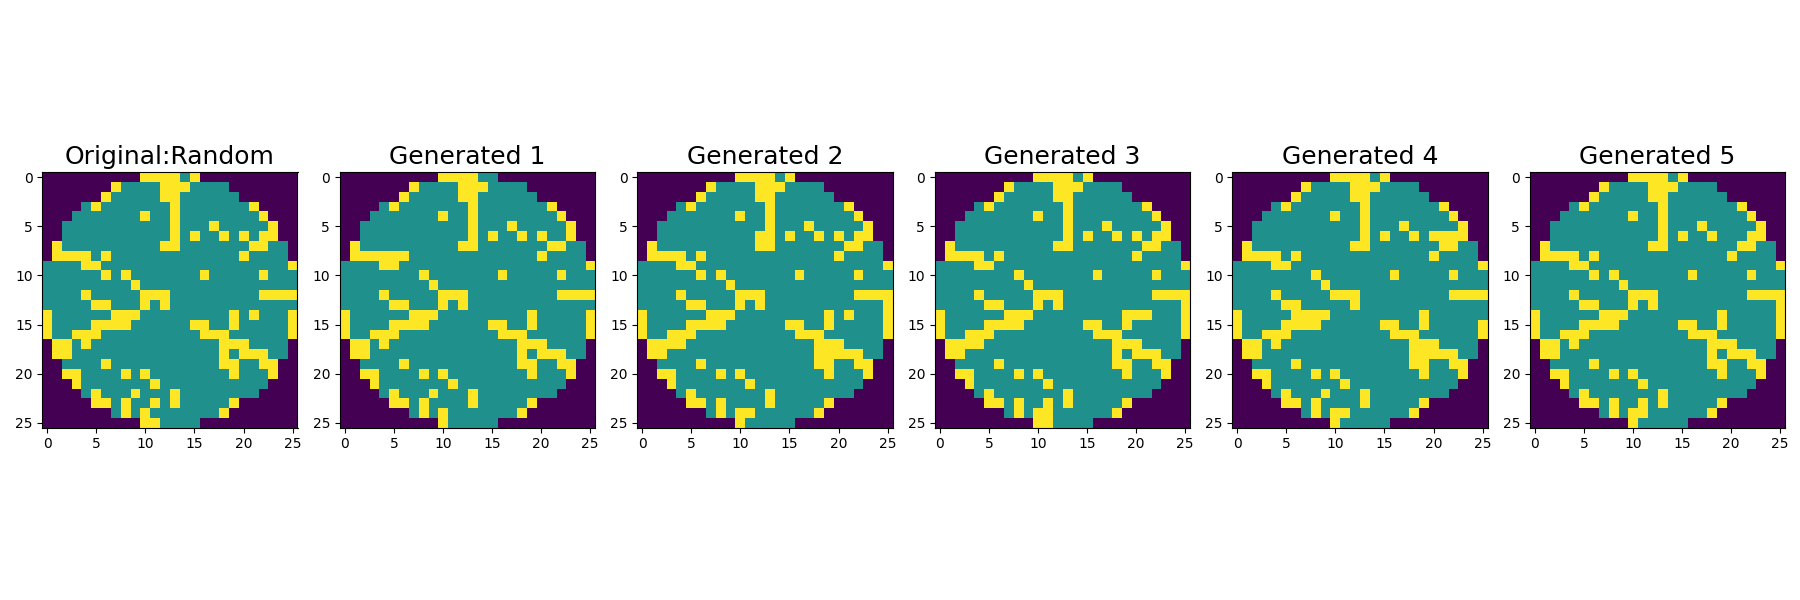
\includegraphics[width=\textwidth]{Random.png}
        \centering
        \caption{Random} \label{fig:11}
    \end{figure}
    \begin{figure}[H]
        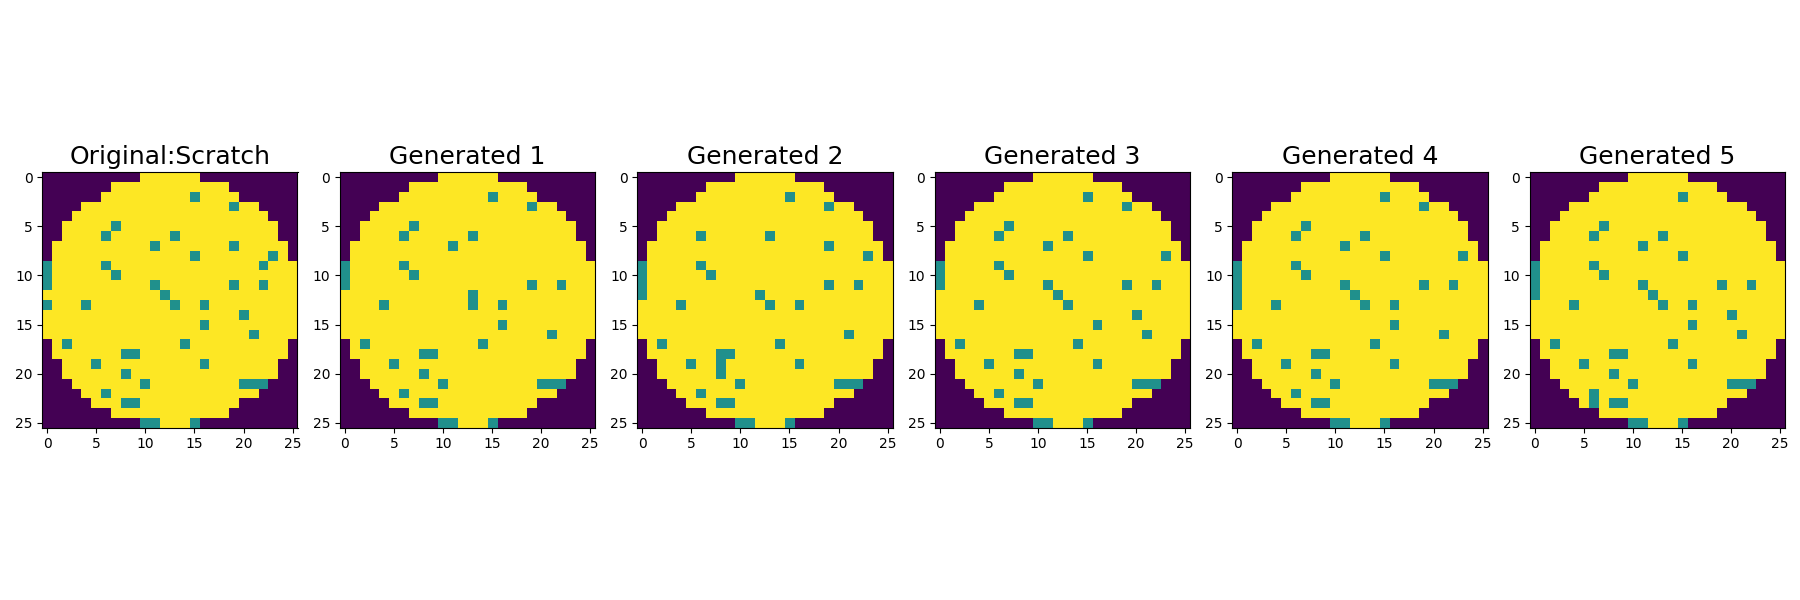
\includegraphics[width=\textwidth]{Scratch.png}
        \centering
        \caption{Scratch} \label{fig:12}
    \end{figure}
\end{document}
